\documentclass[tikz,png]{standalone}
\usepackage{unicode-math}
\usetikzlibrary{positioning}
\begin{document}
  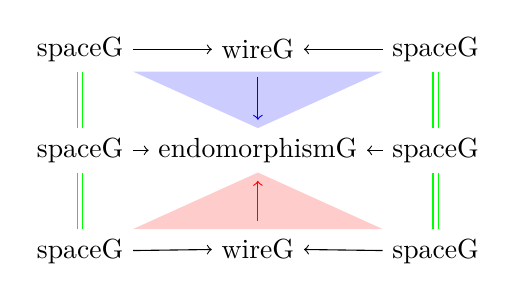
\begin{tikzpicture}
    % r₁
    \node (r1w) {wireG};
    \node[left = of r1w] (r1l) {spaceG};
    \node[right = of r1w] (r1r) {spaceG};
    \draw[->] (r1l) -- (r1w);
    \draw[->] (r1r) -- (r1w);
    % s₀
    \node[below = of r1w.center] (e) {endomorphismG};
    \node[below = of r1l.center] (s0l) {spaceG};
    \node[below = of r1r.center] (s0r) {spaceG};
    \draw[->] (s0l) -- (e);
    \draw[->] (s0r) -- (e);
    % r₀
    \node[below = of e.center] (r0w) {wireG};
    \node[below = of s0l.center] (r0l) {spaceG};
    \node[below = of s0r.center] (r0r) {spaceG};
    \draw[->] (r0l) -- (r0w);
    \draw[->] (r0r) -- (r0w);
    % forward cone
    \fill[fill=red!20] (r0l.north east) -- (e.south) -- (r0r.north west);
    % forward rewrite
    \draw[red,->,shorten >=3pt,shorten <=3pt] (r0w) -- (e);
    % backward cone
    \fill[fill=blue!20] (r1l.south east) -- (e.north) -- (r1r.south west);
    % backward rewrite
    \draw[blue,->,shorten >=3pt,shorten <=3pt] (r1w) -- (e);
    % equalities between regular heights
    \draw[green,double equal sign distance] (r1l) -- (s0l);
    \draw[green,double equal sign distance] (r1r) -- (s0r);
    \draw[green,double equal sign distance] (r0l) -- (s0l);
    \draw[green,double equal sign distance] (r0r) -- (s0r);
  \end{tikzpicture}
\end{document}
